\usepackage{graphicx}

% !Mode:: "TeX:UTF-8"
% Author: Zhengxi Tian
% Email: zhengxi.tian@hotmail.com

\chapter{绪论}\label{ch:绪论}

\section{课题研究背景}\label{sec:课题研究背景}
早期的对话系统的用途主要是帮助用户用自然语言使用某个系统,比如预订机票、预订餐馆的座位、查询航班等。这一类系统又被称为任务导向的系统,其早期的实现技术包括关键词匹配、规则和模板以及对话状态追踪,需要大量人工标注的数据等等。这些系统往往只能处理特定领域内的对话,不能回答开放性问题,用途比较局限。

随着在线聊天的盛行,社交媒体和互联网论坛积聚了大量的聊天语料数据,具有代表性的社交媒体和论坛有推特(Twitter),Reddit和微博。大量的数据使人们可以构建开放领域的,面向闲聊的对话系统,这种系统的主要用途是娱乐、语言教育和陪伴,能根据和对话的上下文和用户的提问产生语义相关的回答。这种系统的文献主要考察二人对话,两人聊天的历史记录称为上下文(context),记为$c$;当前说话的人说出的话语称为消息(message),记为$m$;另外一个人对该消息的回复称为响应(response),记为$r$。$c,m,r$三者的关系如图~\ref{fig:context_message_response}所示。系统的输入是$c,m$,输出是$r$,也就是把对话的上下文和消息映射为响应,这个问题称为对话响应生成(Conversation Response Generation),简称响应生成。

\begin{figure}[H]
    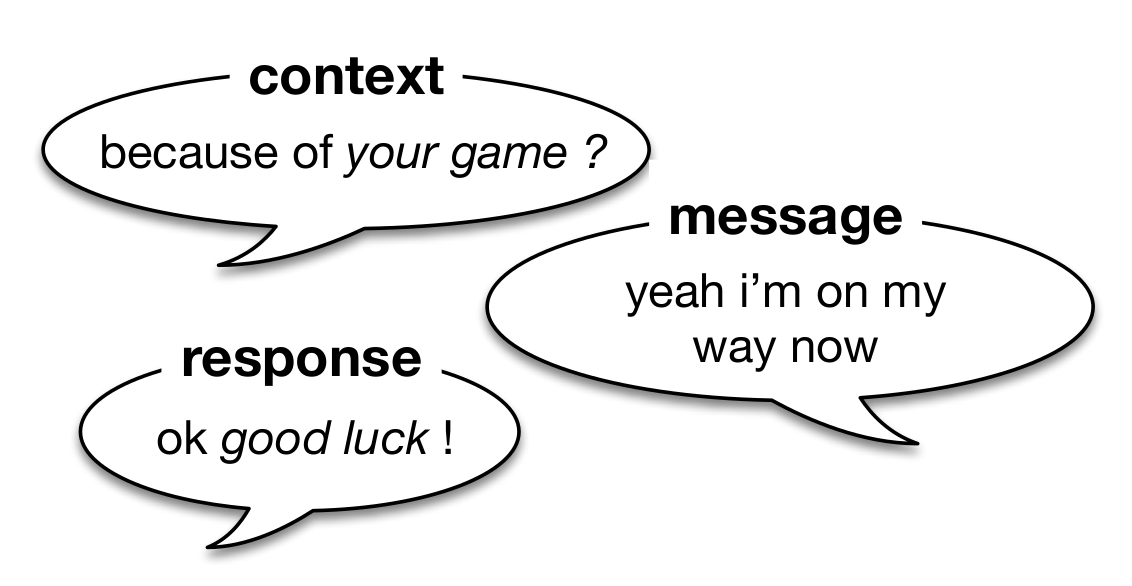
\includegraphics[width=0.6\textwidth]{figure/context_message_response.png}
    \centering
    \caption{上下文,消息和响应的关系
    \upcite{DBLP:journals/corr/SordoniGABJMNGD15}}
    \label{fig:context_message_response}
\end{figure}

Ritter等人率先用统计机器翻译(Statistical Machine Translation,SMT)的方法\upcite{Ritter:2011:DRG:2145432.2145500}解决响应生成问题。他们没有考虑上下文,而是把一个消息直接翻译为响应。Sordoni等人首次把神经网络用于响应生成,用神经网络对SMT输出的响应进行重现排序\upcite{DBLP:journals/corr/SordoniGABJMNGD15}。他们的模型属于在机器翻译中非常有效的编码器-解码器架构(Encoder-Decoder),对输入的上下文和消息进行词袋化(Bag-of-Word)后,用一个前馈神经网络(Feed-Forward Neural Network)进行编码,再用一个朴素的\footnote{称其为朴素的是因为它没有使用LSTM或者GRU,仅用了$\sigma$激活函数。}(Recurrent Neural Network,RNN)构成的语言模型(Language Model,LM)\upcite{DBLP:conf/interspeech/MikolovKBCK10}进行解码,根据上下文和消息的特征组合方式不同,他们提出了三个模型:RLM,DCGM-1和DCGM-2。Sutskever等人于2014年提出了基于RNN的编解码器,也就是序列到序列架构(Seq2Seq)\upcite{DBLP:conf/nips/SutskeverVL14}。

\begin{figure}[H]
    \centering
    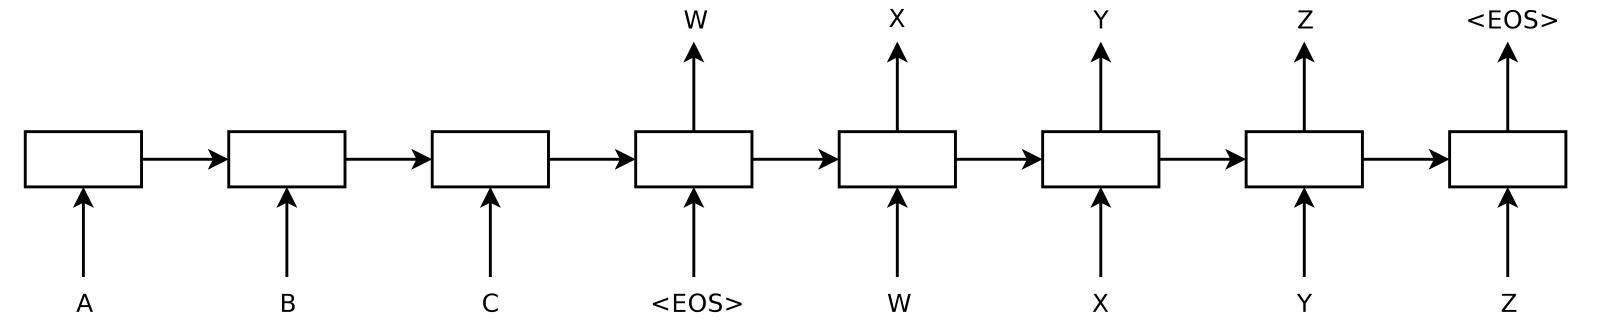
\includegraphics[width=0.8\textwidth]{figure/Seq2Seq.png}
    \caption{Seq2Seq架构图\upcite{DBLP:conf/nips/SutskeverVL14}}
    \label{fig:Seq2Seq}
\end{figure}

\section{课题研究意义}\label{sec:课题研究意义}


\section{课题研究内容}\label{sec:课题研究内容}


\section{论文组织结构}\label{sec:论文组织结构}
本文剩下的组织结构是这样的:第二章《相关工作》总结了领域内对自动化指标的使用和研究现状,主要列举了生成式对话系统最为常用的
几个自动化指标:BLEU,困惑度(Perplexity,PPL),基于词嵌入的指标(Embedding Based)和研究者为了衡量对话的多样性而提出的
指标,如DeltaBLEU,ADEM,RUBER和LSDSCC等。本文的第三章《研究方法》介绍了本次实验所使用的框架,包括对涉及到的模型、数据集和
指标的简介,框架的运行流程,以及实验设计的数学依据。本文的第四章《实验结果与讨论》详细的介绍了所有实验的细节,包括模型训练的参数,数据集的预处理,
最重要的是,实验数据的分析和呈现。我们将从数据中分析得出几个重要的结论。最后一章是《总结》,我们总结实验所得出的结论并给出了
生成式模型的自动化指标的几个发展方向。
